\documentclass[17pt,a4paper,landscape]{extarticle}
\usepackage[margin=2.35cm]{geometry}
\usepackage{amsmath}
\usepackage{amssymb}
\usepackage{tasks}
\usepackage{tikz}
\usepackage{xcolor}
\usepackage[sfdefault,lf]{FiraSans}
\renewcommand{\familydefault}{\sfdefault}
\setlength{\parindent}{0pt}
\pagestyle{empty}
\settasks{label=\textbf{\arabic*.}, label-width=2.2em, item-indent=2.95em, column-sep=2.1cm, after-item-skip=7.8em}
\renewcommand{\arraystretch}{1.15}
\everymath{\displaystyle}

\begin{document}
\sffamily
\boldmath

\boldmath

\boldmath

\boldmath

\boldmath

\boldmath

\vspace*{0.4em}
{\LARGE \textbf{Foundation}}
\begin{tasks}(3)
\task Write a fraction equivalent to $\frac{1}{2}$.
\task Write a fraction equivalent to $\frac{2}{3}$.
\task Write a fraction equivalent to $\frac{3}{4}$.
\task Write a fraction equivalent to $\frac{4}{5}$.
\task Are $\frac{1}{2}$ and $\frac{2}{4}$ equivalent?
\task Are $\frac{3}{5}$ and $\frac{6}{10}$ equivalent?
\task Fill in the blank: $\frac{1}{3} = \frac{\square}{6}$
\task Fill in the blank: $\frac{2}{5} = \frac{\square}{10}$
\task Fill in the blank: $\frac{3}{4} = \frac{\square}{8}$
\task Fill in the blank: $\frac{4}{7} = \frac{8}{\square}$
\task {
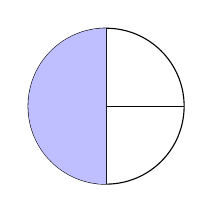
\begin{tikzpicture}[scale=0.9]
\draw (0,0) circle (1.1);
\draw (0,0)--(90:1.1);
\draw (0,0)--(180:1.1);
\draw (0,0)--(270:1.1);
\draw (0,0)--(0:1.1);
\fill[blue!25] (0,0)--(90:1.1) arc (90:180:1.1)--cycle;
\fill[blue!25] (0,0)--(180:1.1) arc (180:270:1.1)--cycle;
\end{tikzpicture}
}
\task {
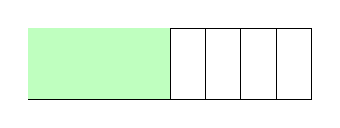
\begin{tikzpicture}[scale=0.9]
\draw (0,0) rectangle (4,1);
\foreach \x in {1,2,3} \draw (\x,0)--(\x,1);
\foreach \x in {0,0.5,...,4} \draw (\x,0)--(\x,1);
\fill[green!25] (0,0) rectangle (2,1);
\end{tikzpicture}
}
\end{tasks}

\end{document}
